\documentclass{article}
\usepackage{amsmath}
\usepackage{fancyhdr}
\usepackage{amsmath}
\usepackage{clrscode}
\usepackage{subfigure}
\usepackage[top=3cm, bottom=3cm, left=3cm, right=3cm]{geometry}
\usepackage[pdftex]{graphicx}\title{BME511L: Lab4}
\usepackage{float}
\usepackage{amsfonts}
\author{Allen Yin}
\pagestyle{fancy}
\setlength\parindent{0.0in}
\setlength\parskip{0.0in}
\usepackage{caption}
\captionsetup{justification=justified}
\setcounter{tocdepth}{2}
\setlength{\headheight}{15pt}

\begin{document}
\maketitle
\setlength\parskip{0.1in}

\section{1D Fitzhugh-Nagumo Model Active Fiber}
Current is applied from right to left for 5ms. At the end of this interval, the contour of the biodomain transmembrane potential $Vm$, and $Vm$ along the entire strip is shown below:

\begin{figure}[H]
    \begin{center}
        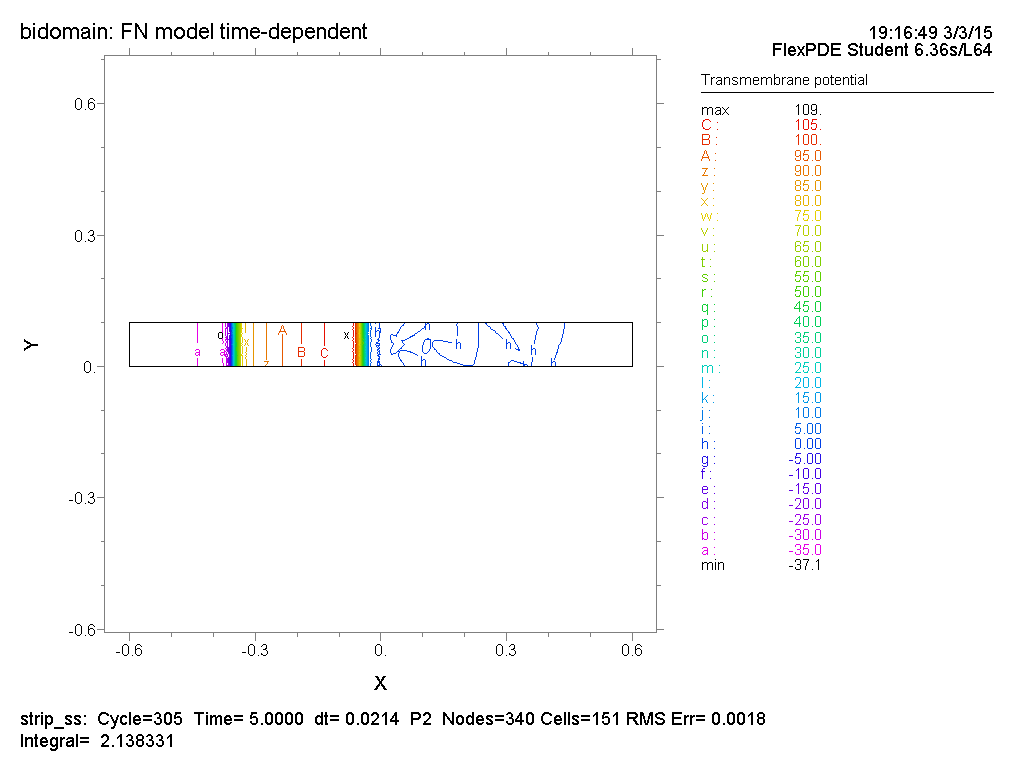
\includegraphics[scale=0.5]{1Dstrip_contourVm_t=5ms.png}
        \caption{Contour plot of $Vm$ at end of 5ms.}
    \end{center}
\end{figure}

\begin{figure}[H]
    \begin{center}
        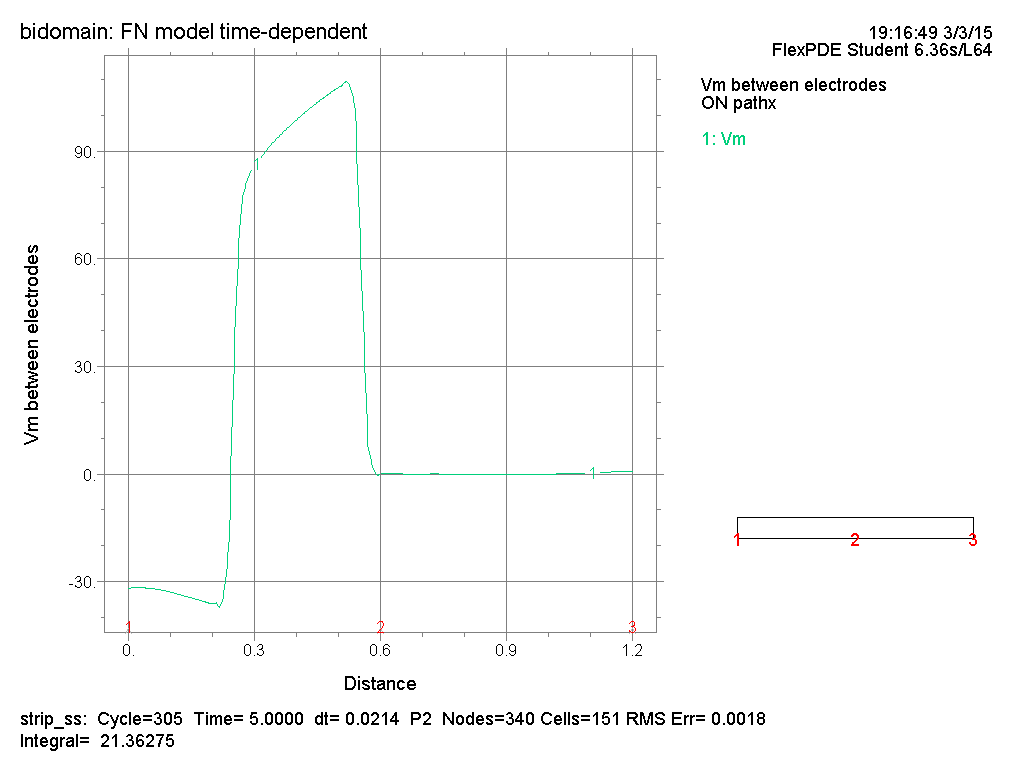
\includegraphics[scale=0.5]{1Dstrip_VmAlongStrip_t=5ms.png}
        \caption{$Vm$ along tissue strip at end of 5ms.}
    \end{center}
\end{figure}

The simulation is ran for another 10ms at the termination of the current stimulus. $Vm$ at the middle of the strip is shown below:

\begin{figure}[H]
    \begin{center}
        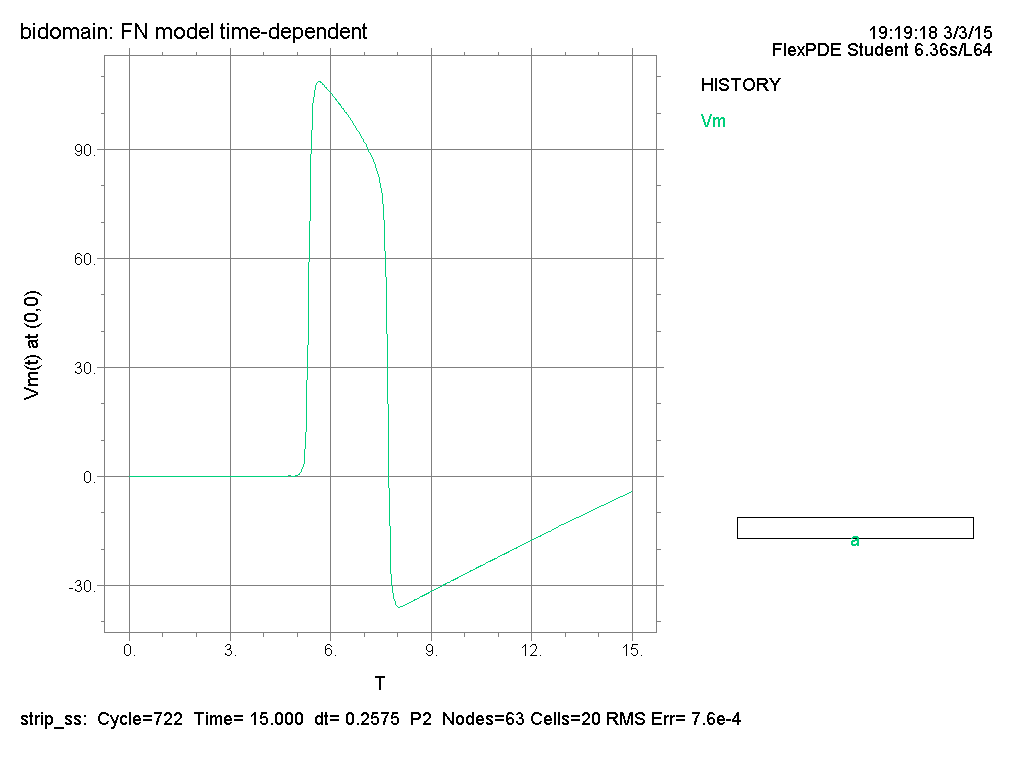
\includegraphics[scale=0.5]{1Dstrip_VmOrigin_tmax=15ms.png}
        \caption{$Vm(t)$ at the middle of the strip for 15ms.}
    \end{center}
\end{figure}

Note that we can observe a full action potential, including the repolarization. The extracellular potential ($\Phi_0(t)$) due to the action potential, measured at an electrode $0.1cm$ above the center of the tissue is shown below. The peak of $Vm(t)$ at the origin corresponds to the minimum of $\Phi_0(t)$.

\begin{figure}[H]
    \begin{center}
        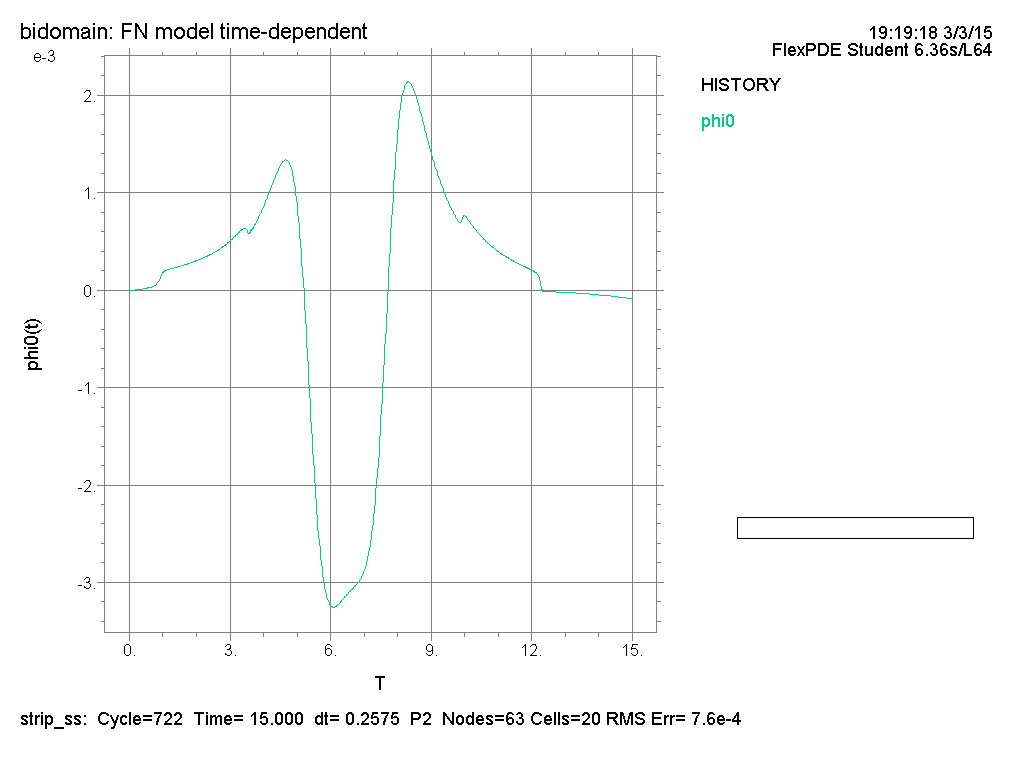
\includegraphics[scale=0.5]{1Dstrip_Phi0_Origin_tmax=15ms.png}
        \caption{$\Phi(t)$}
    \end{center}
\end{figure}

\section{2D Fithugh-Nagumo Model Active Fiber}
Current is applied in the same fashion from electrodes of width $W$. However, the total width of the strip of tissue has now widened to half of its total length. The electrodes now occupy a relatively small part of the width.

At the end of the $5ms$ for which the stimulus is applied, the contour of $Vm$ and $Vm$ along the bottom of the strip is shown below:

\begin{figure}[H]
    \begin{center}
        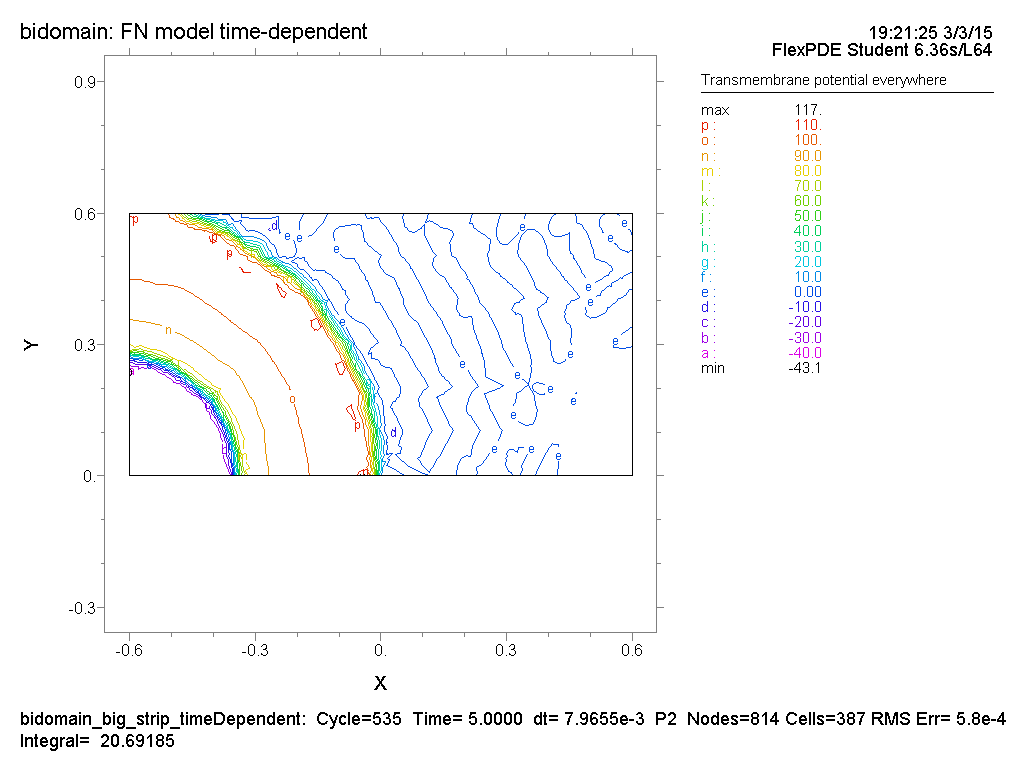
\includegraphics[scale=0.5]{2Dstrip_contourVm_t=5ms.png}
        \caption{Contour plot of $Vm$ at end of 5ms.}
    \end{center}
\end{figure}

The contour lines due to the action potential now propagates diagonally from the left electrode toward top-right, as expected in a 2D tissue.

\begin{figure}[H]
    \begin{center}
        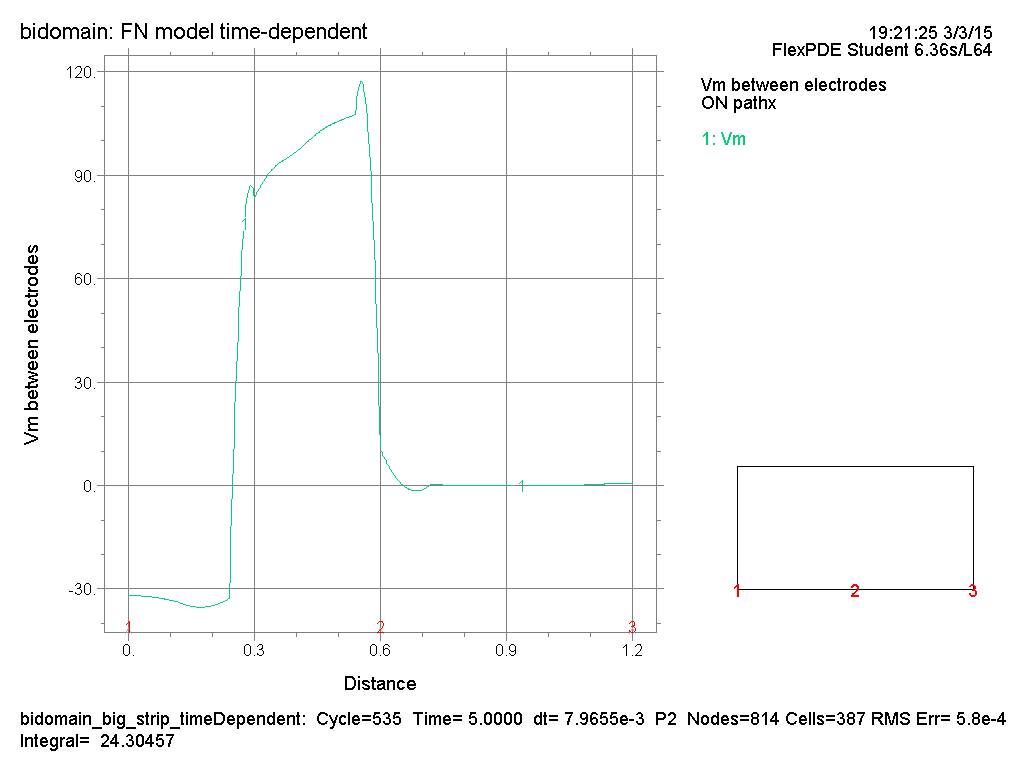
\includegraphics[scale=0.5]{2Dstrip_VmAlongStrip_t=5ms.png}
        \caption{$Vm$ along tissue strip at end of 5ms.}
    \end{center}
\end{figure}

The simulation is ran for another 10ms at the termination of the current stimulus. $Vm$ at the middle of the strip is shown below:

\begin{figure}[H]
    \begin{center}
        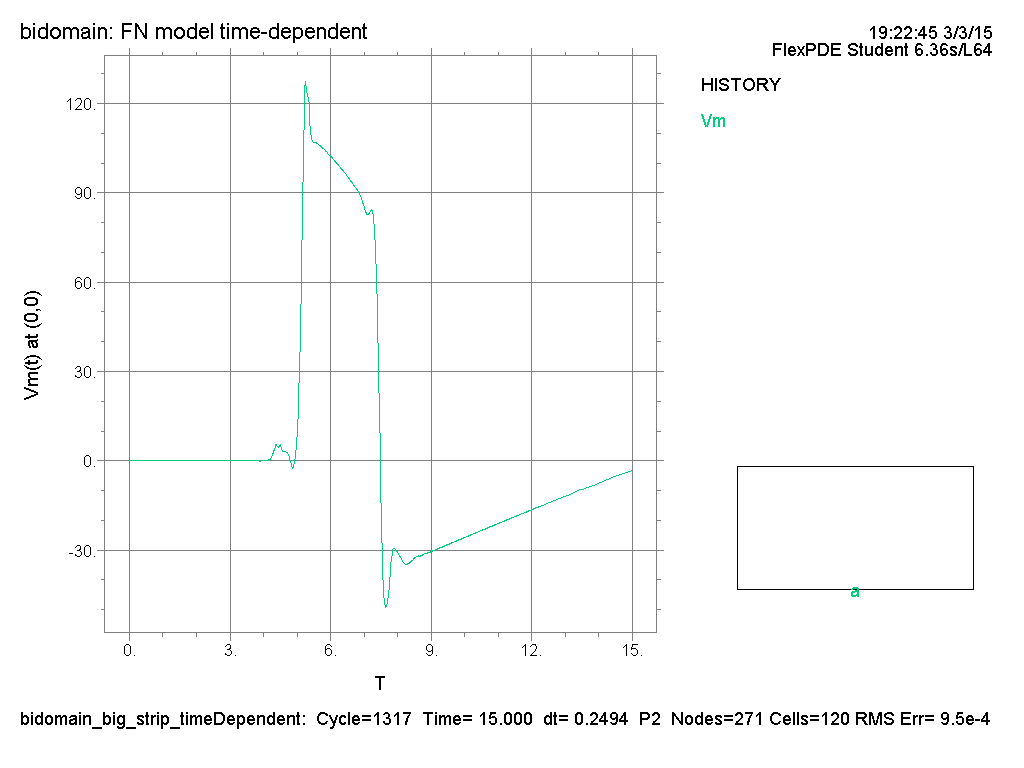
\includegraphics[scale=0.5]{2Dstrip_VmOrigin_tmax=15ms.png}
        \caption{$Vm(t)$ at the middle of the strip for 15ms.}
    \end{center}
\end{figure}

The extracellular potential $\Phi(t)$ measured at $(0,0,0.1cm)$ is also plotted for the time course.

\begin{figure}[H]
    \begin{center}
        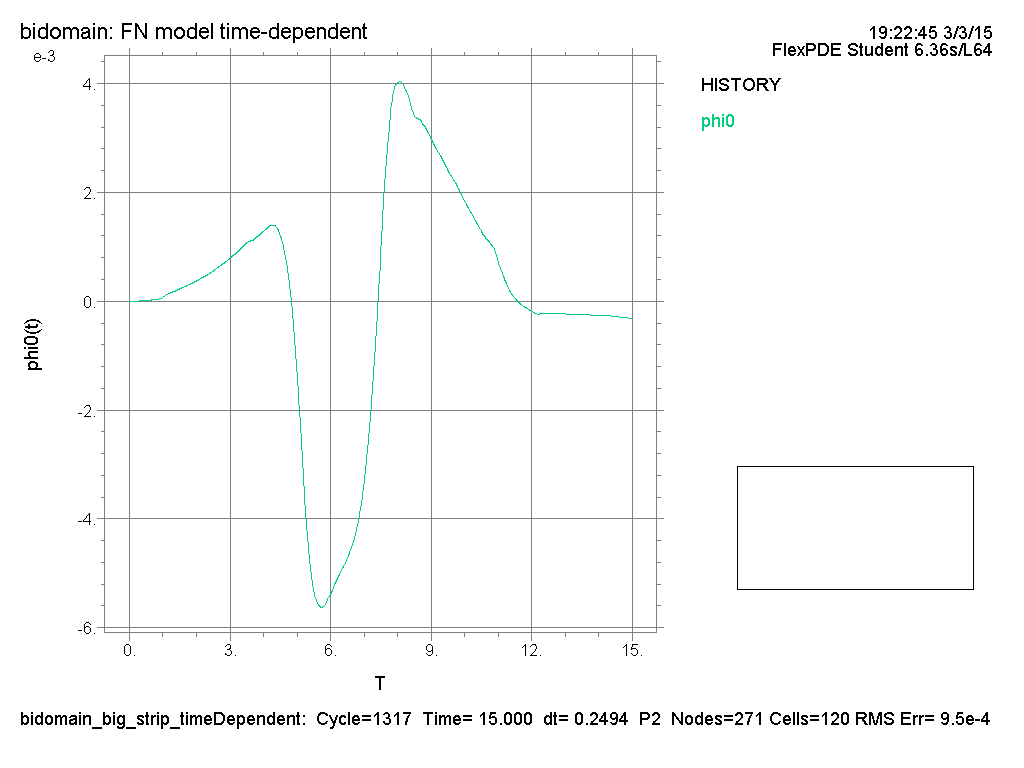
\includegraphics[scale=0.5]{2Dstrip_Phi0_Origin_tmax=15ms.png}
        \caption{$\Phi(t)$}
    \end{center}
\end{figure}

\section{Question 6}
The magnitude of $\Phi_0(t)$ of the 2D fiber is roughly twice that of the 1D fiber. This is expected since the volume of tissue in the 2D tissue is roughly 6 times that of the 1D tissue. This makes sense since $\Phi_0(t)$ scales with the conducting volume.

To confirm the order of magnitude of $\Phi_0(t)$ in the 1D case, we start with the formula:
\[\Phi_0 = \frac{-1}{4\pi\sigma_0}\frac{g_ig_e}{g_i+g_e}\int_V\nabla V_m\cdot\nabla(\frac{1}{r})dv\].

The constant outside of the integral is dimensionless and is about $-0.00335$. The term inside the order of $(100mV/cm)*(\frac{1}{0.1cm})^2=10000mV/cm^3$. The total volume of the tissue is $1.2cm*0.1cm*18\mu m=0.000216cm^3$. Multiplying these two together, we get the integral to be about $2.16mV$. Thus $\Phi_0\approx 7.236\times10^{-3}mV$, which is the same order of magnitude as the simulation results.

\section{Question 7}
Looking at the plots, it looks like flexPDE introduces more glitches in the 2D simulation results (visually as peaks in the $Vm(t)$ and $Vm(x)$ plots). This can probably be improved with finer time and spatial resolution.

FlexPDE offers an easy way to model excitable tissue, in terms of ease of programming.

\section{Question 8}
To limit the inaccuracy of calculating $\Phi_0(t)$ in simulations, we decomposed the analytical integral into two parts via integration by parts, making it a difference of two integrals involving only the first gradient of $V_m$. The boundary term in this equation is then discarded to simplify calculations, which then resulted in the glitches in the $\Phi_0(t)$ plots.

\end{document}
